\documentclass[11pt,a4paper]{article}

\usepackage[polish]{babel}
\usepackage[utf8]{inputenc}
\usepackage{polski}
\usepackage[T1]{fontenc}
\usepackage{indentfirst}
\usepackage{wrapfig}    % for wrapping figures, tables

\frenchspacing

%\usepackage{amsmath}
\usepackage{physics}
%\usepackage{bm}
\usepackage{gensymb}
%\usepackage{hepnames}
\usepackage{epsfig}
\usepackage{graphics}
\usepackage[shortlabels]{enumitem}
%\usepackage{xspace}
%\xspaceaddexceptions{[]\{\}}

%
%
%fixpagesize
\pagestyle{empty}
\addtolength{\textwidth}{6cm}
\addtolength{\textheight}{4cm}
\addtolength{\evensidemargin}{-3cm}
\addtolength{\oddsidemargin}{-3cm}
\addtolength{\topmargin}{-2cm}
\parindent=0cm


%
%
%small distance in list/item/enum for enumitem package
\setlist[itemize,enumerate]{topsep=0em}
\setlist{noitemsep}

%print zadanie #
\newcounter{zadanie}\newcommand{\zadanie}[1][]{\addtocounter{zadanie}{1} ~\\  {\bf \emph{Zadanie \arabic{zadanie} #1 }} \\}
\newcounter{zaddom}\newcommand{\zaddom}[1][]{\addtocounter{zaddom}{1} ~\\  {\bf \emph{Zadanie domowe \arabic{zaddom} #1 }} \\}
%\renewcommand{\zadanie}[1][]{\pagebreak  ~\\  {\bf \emph{Zadanie }} \\} \addtolength{\topmargin}{-2cm}

\newcommand{\dbar}{{\mkern3mu\mathchar'26\mkern-12mu d}}


%%%%%%%%%%%%%%%%%%%%%%%%%%%%%%%%%%%%%%%%%%%%%%%%%%%%%%
\begin{document}           % End of preamble and beginning of text.

\begin{centering}
\bf{\Large{Termodynamika z elementami fizyki statystycznej}}\\
Tydzień 10 (4 maja 2023)\\[3mm]
Entropia i cykle w T-S\\
\end{centering} 
\vspace{5mm}

\zadanie
Znajdź sprawność cyklu Carnota rozważając go we współrzędnych $T-S$.
Wykaż, że sprawność silnika Carnota jest maksymalna.

\zadanie
Narysuj we współrzędnych $T-S$ cykl Stirlinga (dwie izotermy, dwie izochory) 
oraz oblicz jego sprawność (z regeneracją i bez).
Porównaj z cyklem Carnota.

\zadanie
Obliczyć sprawność silnika cieplnego, którego cykl we współrzędnych $T-S$ jest trójkątem
prostokątnym którego podstawa jest zadana przez 
izotermę $T_1$, a wysokość przez adiabatę (między $T_1$ i $T_2$),  trzeci proces domyka trójkąt.
Wynik podać jako funkcję $T_1$ i $T_2$.\\


\zadanie
Zbiornik zawiera $100\,$kg wody o temperaturze $T_1 = 100^\circ$C.
Znajdź maksymalną pracę, jaką może wykonać maszyna cieplna pracująca pomiędzy tym zbiornikiem a otoczeniem o temperaturze $T_2 = 0^\circ$C.
Założyć, że w trakcie całego procesu rozkład temperatury wewnątrz zbiornika jest jednorodny.

\zadanie
Dwa zbiorniki zawierają po $100\,$kg wody każdy.
W jednym woda ma temperaturę $T_1=100^\circ$C,
zaś w drugim $T_2 = 0^\circ$C. Jaką maksymalną, całkowitą,  pracę można wykonać
używając jednego zbiornika jako grzejnika a drugiego jako chłodnicy?
Ciepło właściwe wody wynosi $c_w=4200\,{\rm J/(kg\, K)}$.


\pagebreak

\begin{wrapfigure}[6]{r}{0.3\linewidth}\vspace{-8mm}
\resizebox{\linewidth}{!}{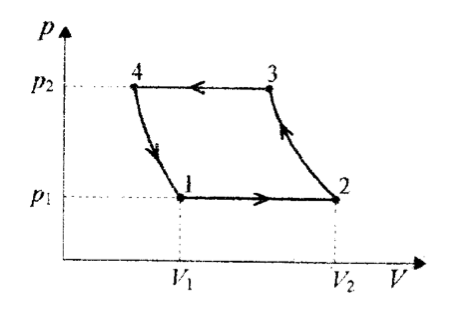
\includegraphics{seria2_rys1.png}}
\end{wrapfigure}
\zaddom
Oblicz, we współrzędnych $T-S$ współczynnik efektywności lodówki, pracującej w oparciu o cykl składający
się z dwóch izobar i dwóch adiabat (rysunek). Dane są: $V_1$, $V_2$, $p_1$ i $p_2$.
Czynnikiem roboczym jest jednoatomowy gaz doskonały. Gaz roboczy jest w kontakcie z lodówką 
jedynie na etapie kiedy pobiera ciepło z otoczenia.

{\it Odpowiedź:} $\eta_L = \frac{1}{\left( \frac{p_2}{p_1}\right)^{\frac{\kappa-1}{\kappa}} -1 }$



\zaddom
Oblicz sprawność silnika opartego na cyklu Otto (tj. dwie izochory, dwie adiabaty)
we współrzędnych $T-S$. Gaz roboczy stanowi $n$ moli gazu doskonałego.
Dane są: ciepło molowe $C_V$, objętości gazu maksymalna: $V_1$ i 
 minimalna: $V_2$.

{\it Odpowiedź:} $\eta_S = 1 - \left( \frac{V_2}{V_1}\right)^{\frac{R}{C_V}}$

\vspace*{5mm}

\begin{wrapfigure}[6]{r}{0.25\linewidth}\vspace{-10mm}
\resizebox{\linewidth}{!}{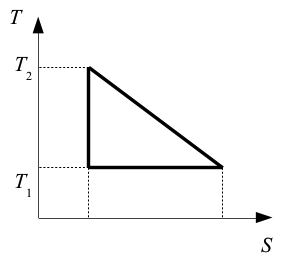
\includegraphics{seria2_rys4.png}}
\end{wrapfigure}
\zaddom
Pompa ciepła wykorzystuje cykl, który jest przedstawiony
we współrzędnych $T-S$ na rysunku obok.
Zaznacz właściwy kierunek cyklu i oblicz sprawność takiej pompy.
Substancją roboczą jest gaz doskonały.
Dane są: $T_2$~i $T_1$ (gdzie $T_2>T_1$).%\\[1mm]

{\it Odpowiedź:} $\eta_P = \frac{T_2 +T_1}{T_2 - T_1}$, obieg przeciwne do ruchu wskazówek zegara. 

\vspace*{5mm}
\zaddom
%{\bf\em lodówka Carnota}\\
Ile co najmniej kilowatogodzin energii elektrycznej trzeba zużyć, aby w, gorący, 
letni dzień schłodzić w lodówce karton soku o masie $m=1\,$kg
od temperatury otoczenia $T_1=30^\circ$C do temperatury końcowej $T_2=5^\circ$C?
Przyjmij, że:
temperatura otoczenia nie zmienia się, ciepło właściwe soku wynosi $c_{w}=4200\,{\rm J/(kg\, K)}$,
karton soku idealnie wypełnia całe wnętrze lodówki,
sprawność konwersji energii elektrycznej na mechaniczną w kompresorze idealnej lodówki wynosi 100\%, 
a lodówka pracuje w chłodniczym cyklu Carnot.

{\it Odpowiedź:} $W=mc_{w}[(T_1 \ln(\frac{T_1}{T_2}) + T_2-T_1)] = 1.27 \cdot 10^{-3}$~kWh.


\end{document}

\begin{wrapfigure}[8]{r}{0.3\linewidth}\vspace{-5mm}
    \resizebox{\linewidth}{!}{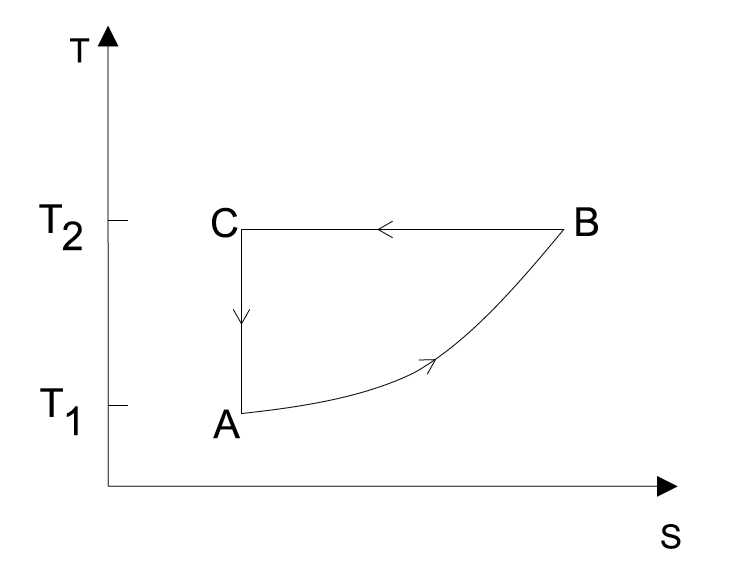
\includegraphics{seria2_rys2.png}}
    \end{wrapfigure}
    %
    \zaddom
    Oblicz sprawność chłodziarki, której cykl we współrzędnych $T-S$
    przedstawiony jest na rysunku. Wiadomo, że: substancją roboczą jest jednoatomowy gaz doskonały, krzywa $AB$ jest izochorą, temperatura $T_1 = 5^\circ$C, a temperatura
    $T_2 = 50^\circ$C.\\[3mm]
    {\em Wskazówka: znajdź równanie adiabaty we współrzędnych $T-V$ dla
    gazu doskonałego.}
    
    {\it Odpowiedź:}  $\eta_L = \frac{T_2-T_1}{T_2 \ln{\frac{T_2}{T_1}}- (T_2 -T_1)}$